\documentclass[
	paper=a4,				% Papierformat
	twoside=true,			% Zweiseitiges Layout
	BCOR=6mm,				% Rand zum Binden
	fontsize=12pt,			% Schriftgröße
	pagesize=auto,			% Schreibt die Papiergröße korrekt ins Ausgabedokument
	numbers=noenddot,		% Kein Punkt nach der Kapitel-Nummer
	bibliography=totoc,		% Quellenverzeichnis im Inhaltsverzeichnis auflisten
	draft=false
]{scrartcl}
% siehe http://tex.stackexchange.com/questions/183149/cant-silence-a-pdftex-pdf-inclusion-multiple-pdfs-with-page-group-error
\pdfsuppresswarningpagegroup=1
% Legt die Zeichenkodierung fest, z.B UTF8
\usepackage[utf8]{inputenc}
% Erweiterten Zeichensatz für europäische Sprachen aktivieren
\usepackage[T1]{fontenc}
% Silbentrennung nach neuer deutscher Rechtschreibung
\usepackage[ngerman]{babel}
% Beseitigt Probleme mit noch nicht vollständig aktualisierten Paketen (z.B. listings)
\usepackage{scrhack}
% Zum flexiblen Einbinden von Grafiken, pdftex ist optional
\usepackage[pdftex]{graphicx}
% Umgebung um mehrere Abbildungen zu einer zu kombinieren
\usepackage{subfig}
% Führt die SCfigure-Umgebung ein (Caption neben der Abbildung)
\usepackage{sidecap}
\renewcommand{\sidecaptionrelwidth}{2.0}
% Damit kann ein Bild vom Text umflossen werden
\usepackage{wrapfig}
% Darstellung für Caption s.u.
\usepackage[font=small,labelfont=bf,labelsep=colon,format=plain]{caption}
\usepackage{amsmath}
\usepackage{amssymb}
\usepackage{cite}
% Verbessert die Kompatibilität von siunitx mit microtype
\usepackage{textcomp}
\usepackage{siunitx}
\sisetup{
	output-decimal-marker = {,},
	per-mode = symbol,
	list-final-separator = { und },
	list-pair-separator = { und },
	range-phrase = { bis },
}
\usepackage{listings}
% Umlaute in Listings sind nur mit folgender Option möglich:
\lstset{
    literate={ö}{{\"o}}1
    {ä}{{\"a}}1
    {ü}{{\"u}}1
}
% Standard-Werte für Listings festlegen:
\lstset{
    frame=single,
    flexiblecolumns=true,
    commentstyle=\color{darkgreen},
    float,
    basicstyle=\small\sffamily,
    numbers=left,
    numberstyle=\tiny,
    showstringspaces=false,
    keepspaces,
    tabsize=4
}
% Zum Einfärben von Code:
\usepackage{color}
\definecolor{darkgreen}{rgb}{0,0.5,0}

% Fußnoten formatieren und Unterstützung für aufeinander folgende Fußnoten:
\usepackage[flushmargin,multiple]{footmisc}
% Hurenkinder und Schusterjungen komplett verbieten:
%\clubpenalty = 10000
%\widowpenalty = 10000
%\displaywidowpenalty = 10000
%\usepackage{microtype}
% Hyperlinks erstellen, wobei Fußnoten aus Kompatibilitätsgründen ausgenommen werden:
\usepackage[hyperfootnotes=false,pdfpagelabels]{hyperref}

% subsubsections werden nummeriert (Standard: subsections)
\setcounter{secnumdepth}{\subsubsectionnumdepth}

% Platz für 3 stellige Seitenzahlen im Inhaltsverzeichnis schaffen:
\makeatletter
\renewcommand{\@pnumwidth}{3em} 
\renewcommand{\@tocrmarg}{4em}
\makeatother

% Schriftgröße der Bildunterschriften verkleinern:
\addtokomafont{caption}{\small\linespread{1}\selectfont}
% Zweite Zeile der Bildunterschrift einrücken:
\setcapindent{1em}

\begin{document}	

\author{Michael Entrup}
\title{Anhang C \\ Das Auflösungsvermögen von ESI}
\date{April 2017}

\maketitle

% Inhaltsverzeichnis
\tableofcontents

\section{Motivation}

Die Linsen in einem Elektronenmikroskop weisen diverse Abbildungsfehler auf, die zu einer Reduzierung der Ortsauflösung führen. Möchte man hoch aufgelöste Messungen mit dem Elektronenmikroskop aufnehmen, so sollte man das theoretische Auflösungsvermögen kennen und sich den Parametern bewusst sein, die Einfluss auf das Auflösungsvermögen haben. Im folgenden Abschnitt soll eine Herleitung für das theoretische Auflösungsvermögen präsentiert werden, die mit dem SageMath implementiert wurde. Der entsprechende Programmcode ist auf \url{https://github.com/m-entrup/Dissertation} im Unterordner \texttt{Jupyter-Notebooks/AnhangC/} zu finden.

Im zweiten Teil dieses Anhangs soll kurz darauf eingegangen werden, welche weiteren Einflüsse zusätzlich das Auflösungsvermögen von ESI bestimmen. Dabei wird insbesondere die Objektivblende betrachtet und welche Auswirkung die Wahl der Blende auf die resultierende Intensität auf das energieselektive Bild besitzt.

\clearpage

\section{Das Auflösungsvermögen berechnen}

Durch die Verwendung von Elektronen erreicht man mit dem TEM Wellenlängen, die weit unterhalb denen von Licht liegen. Bei einem TEM mit einer Beschleunigungsspannung von \SI{200}{kV} erreicht man eine Wellenlänge von etwa \SI{2,51}{pm}. Nach dem Rayleigh-Kriterium beträgt somit das Auflösungslimit $\frac{\num{0,61}\cdot\lambda}{\sin\alpha}\approxeq\SI{1,53}{pm}$. Dies ist um den Faktor 65 geringer als die in \cite{tanaka_present_2008} erwähnten $\SI{0,1}{nm}=\SI{100}{pm}$. Schuld an dieser deutlich schlechtere Auflösung sind die Abbildungsfehler der benutzten Objektivlinse. Der Öffnungsfehler $C_S$ sorgt dafür, dass Elektronen, welche auf den Außenbereich der Objektivlinse treffen stärker gebeugt werden. Der Brennpunkt dieser Elektronen liegt näher an der Linse, als der Brennpunkt von Elektronen, welche zentral auf die Linse treffen. Anders ausgedrückt entsteht in der Brennebene der Linse eine Fehlerscheibe, dessen Radius mit dem Akzeptanzwinkel der Objektivlinse steigt:

\begin{align}
r_S = M \cdot \text{C}_\text{S}\cdot\alpha^3
\end{align}

Dabei ist $M$ der Vergrößerung, $C_S$ die Öffnungsfehlerkonstante (sphärischen Aberration) und $\alpha$ der Öffnungswinkel der Objektiv-Aperatur. Dieser Radius bezieht sich auf die Bildebene der Objektivlinse. Wir möchten jedoch die Objektebene der Linse betrachten und nutzen deshalb:

\begin{align}
\delta_S = \text{C}_\text{S}\cdot\alpha^3 \label{eq:delta_S}
\end{align}

Da $C_S$ bei Mikroskopen ohne $C_S$-Korrektur in der Größenordnung von \SI{1}{mm} ist, darf der maximale Öffnungwinkel \SI{10}{mrad} betragen, um eine Öffnungsfehlerscheibe mit einem Radius von unter \SI{1}{nm} zu erhalten.

Ein weiteres Problem stellt der Beugungsfehler dar. Verkleinert man den Öffnungswinkel, um die Auswirkungen der sphärischen Aberration zu reduzieren, steigert man gleichzeitig die Auswirkungen durch die Beugung der Elektronen an der verwendeten Lochblende. Aus dem Rayleigh-Kriterium ergibt sich für sehr kleine Winkel:

\begin{align}
\delta_B = \frac{\num{0,61}\cdot\lambda}{\sin\alpha} \approxeq \frac{\num{0,61}\cdot\lambda}{\alpha} \label{eq:delta_B}
\end{align}

Mit Hilfe von Gaußscher-Fehlerfortpflanzung ergibt sich daraus die folgende Gleichung (siehe auch \cite[S.\,28]{thomas_analytische_2013}):

\begin{align}
\delta = \sqrt{\left(\frac{\num{0,61}\cdot\lambda}{\alpha}\right)^2 + \left(\text{C}_\text{S}\cdot\alpha^3\right)^2}\label{eq:delta_TG}
\end{align}

Die Wellenlänge von Elektronen lässt sich mit Hilfe von

\begin{align}
\lambda = \frac{2\pi\si{\planckbar}}{\sqrt{E \left( 2 \cdot \si{\electronmass} + \frac{E}{\si{\clight^2}}\right)}}
\end{align}

berechnen. Dabei ist $E$ die kinetische Energie der Elektronen und \si{\electronmass} deren Ruhemasse. Setzt man $\frac{\mathrm d\delta}{\mathrm d\alpha} = 0$, lässt sich der Winkel $\alpha_{opt}$ bestimmen, bei dem der Radius der Fehlerscheibe minimal und somit das Auflösungsvermögen maximal ist:

\begin{align}
\alpha_{opt} = \num{0,77} \cdot \sqrt[4]{\frac{\lambda}{C_S}} \label{eq:alpha_opt}
\end{align}

Eingesetzt in Gleichung \ref{eq:delta_TG} ergibt sich damit

\begin{align}
\delta_{min} = \num{0,9} \cdot \sqrt[4]{C_S\cdot \lambda^3}\,. \label{eq:delta_min}
\end{align}

\begin{figure}
	\centering
	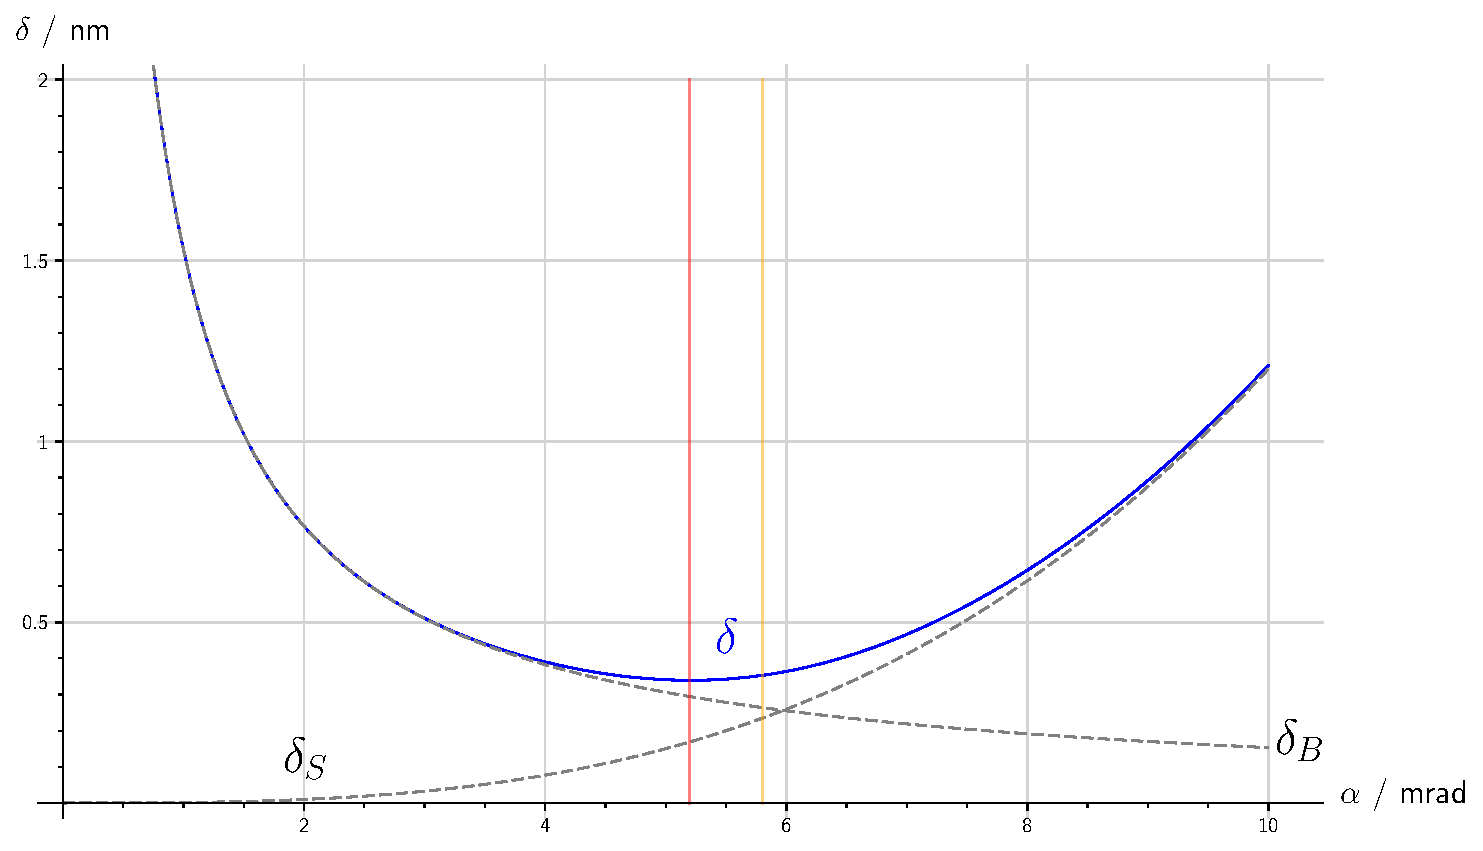
\includegraphics[width=1\linewidth]{../Jupyter-Notebooks/AnhangC/Bilder/delta_TG}
	\caption{Radius der Fehlerscheiben für Öffnung- und Beugungsfehler in Abhängigkeit vom Öffnungswinkel $\alpha$ (Parameter: $C_S = \SI{1,2}{mm}$, $E=\SI{200}{keV}$ und somit $\lambda\approxeq \SI{2,51}{pm}$). Die rote Linie markiert das Minimum von $\delta$. Mit der orangefarben Linie ist das auf Grund der diskreten Blendendurchmesser erreichbare Minimum markiert.}
	\label{fig:delta_TG}
\end{figure}

\begin{figure}
	\centering
	\subfloat[$\delta E = \SI{0,7}{eV}$]{%
		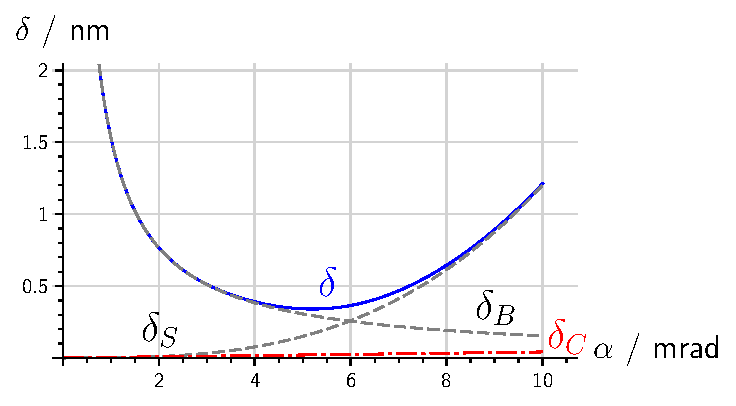
\includegraphics[width=.49\textwidth]{../Jupyter-Notebooks/AnhangC/Bilder/delta_TG_0,7eV}
		\label{fig:delta_TG_0,7eV}
	}
	\subfloat[$\delta E = \SI{20}{eV}$]{%
		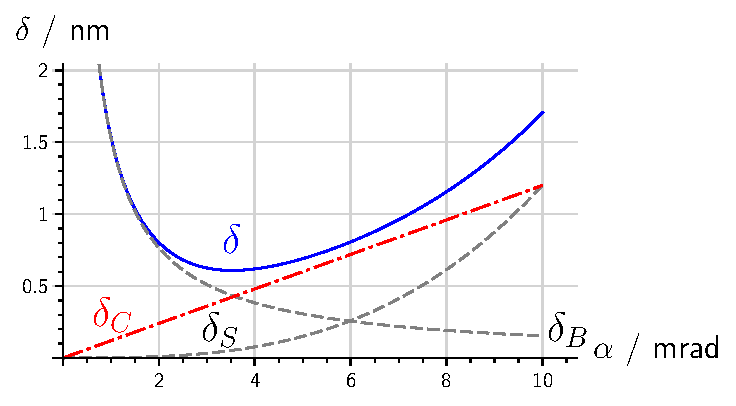
\includegraphics[width=.49\textwidth]{../Jupyter-Notebooks/AnhangC/Bilder/delta_TG_20eV}
		\label{fig:delta_TG_20eV}
	}
	\caption{Radius der Fehlerscheiben für Öffnung-, Beugungs- und Farbfehler in Abhängigkeit vom Öffnungswinkel $\alpha$ (Parameter: $C_S = \SI{1,2}{mm}$, $C_C = \SI{1,2}{mm}$, $E=\SI{200}{keV}$ und somit $\lambda\approxeq \SI{2,51}{pm}$).}
\end{figure}

Alle Aufnahmen für diese Arbeit wurden an einem Zeiss Libra 200FE durchgeführt, das mit einer Beschleunigungsspannung von \SI{200}{kV} arbeitet ($\lambda\approxeq\SI{2,51}{pm}$) und eine Öffnungsfehlerkonstante von $C_S=\SI{1,2}{mm}$ besitzt. Daraus ergibt sich nach Gleichung \ref{eq:alpha_opt} ein optimaler Öffnungswinkel von $\alpha_{opt}\approxeq\SI{5,2}{mrad}$ und damit $\delta_{min}\approxeq\SI{0,33}{nm}$. Der Öffnungswinkel lässt sich leider nur in diskreten Schritten justieren, die durch die Durchmesser der verfügbaren Objektivblenden vorgegeben sind. $\alpha_{opt}\approxeq\SI{5,2}{mrad}$ entspricht einen Durchmesser von $d_{opt}\approxeq\SI{17,9}{\micro m}$ (bei $f=\SI{1,72}{mm}$). Die am nächsten an diesem Wert liegende Blende besitzt einen Durchmesser von $d=\SI{20}{\micro m}$, womit sich $\alpha=\SI{5,8}{mrad}$ für den Öffnungswinkel und $\delta\approxeq\SI{0,35}{nm}$ für den Radius der Fehlerscheibe ergeben. In Abbildung \ref{fig:delta_TG} sind $\delta$, $\delta_S$ und $\delta_B$ in Abhängigkeit vom Öffnungswinkel dargestellt. Es wurden dabei die Geräteparameter des Zeiss Libra 200FE gewählt. Die beiden vertikalen Linien markieren das theoretisch erreichbare Minimum (rot) und das praktisch zu erzielende Minimum (orange).

Bei der bisherigen Betrachtung des Auflösungsvermögens wurde der Farbfehler noch nicht berücksichtigt. Auch dieser führt zu einer Fehlerscheibe, deren Radius sich mit Hilfe von

\begin{align}
\delta_C = \alpha \cdot C_C \cdot \frac{\delta E}{E} \label{eq:delta_C}
\end{align}

berechnen lässt. Warum man den Farbfehler bei einer elastisch gefilterten Abbildung einer dünnen Probe vernachlässigen kann, lässt sich einfach erläutern: Für diese Art von Abbildung spielt nur der Zero-Loss-Peak (ZLP) eine Rolle, da man mit Hilfe der Spaltblende in der energiedispersiven Ebene, nur diesen selektiert. Die Breite der Spaltblende kann vernachlässigt werden, da sich der Großteil der Intensität auf die Halbwertbreite des ZLP verteilt. Beim Zeiss Libra 200FE beträgt diese etwa $\delta E=\SI{0,7}{eV}$, womit sich für die Fehlerscheibe $\delta_C(\alpha = \SI{5,8}{mrad})=\SI{0,024}{nm}$ berechnen lässt ($C_C = \SI{1,2}{mm}$). Die geringe Auswirkung des Farbfehlers zeigt auch Abbildung \ref{fig:delta_TG_0,7eV}. $\delta$ wird dort mit Hilfe von

\begin{align}
\delta_{ESI} &= \sqrt{\delta_B^2 + \delta_S^2 + \delta_C^2} \\
&=\sqrt{\left(\frac{\num{0,61}\cdot\lambda}{\alpha}\right)^2 + \left(\text{C}_\text{S}\cdot\alpha^3\right)^2 + \left(\alpha \cdot C_C \cdot \frac{\delta E}{E}\right)^2} \label{eq:delta_ESI}
\end{align}

berechnet. Da $\delta_C$ viel kleiner ist als $\delta_B$, bzw.\ $\delta_S$, bleiben die Auswirkungen auf $\delta$ gering. Für $\alpha=\SI{5,8}{mrad}$ vergrößert sich $\delta$ von \SI{0,353}{nm} auf \SI{0,354}{nm}.

\begin{figure}
	\centering
	\subfloat[Ohne Berücksichtigung des Öffnungsfehlers]{%
		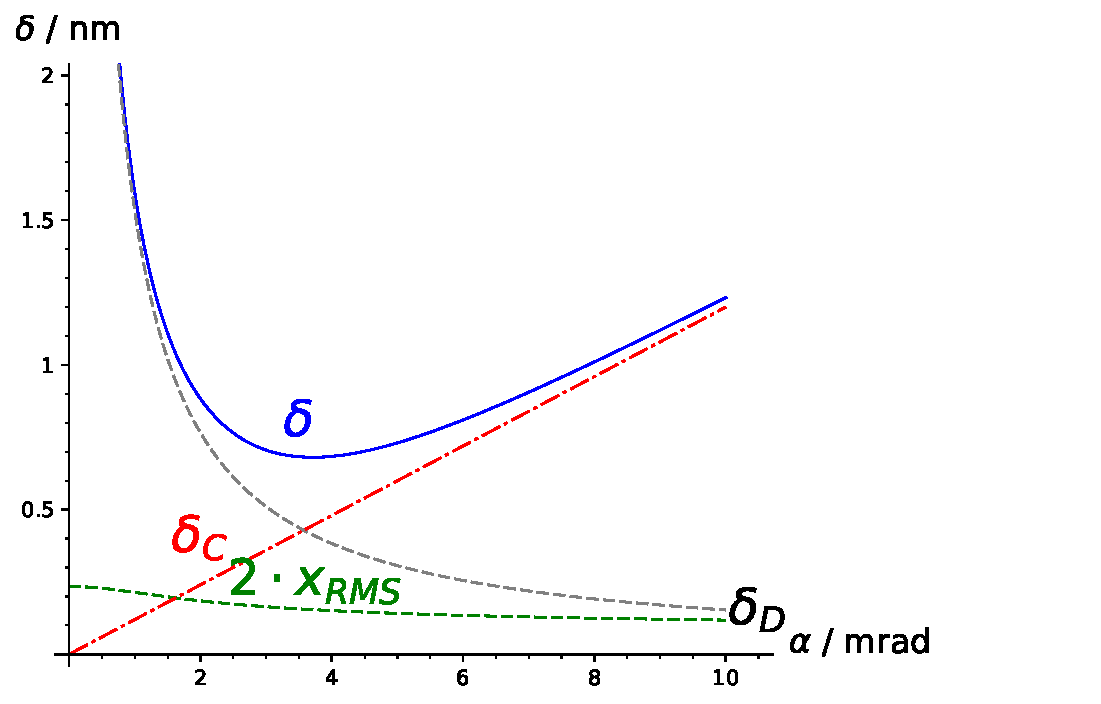
\includegraphics[width=.49\textwidth]{../Jupyter-Notebooks/AnhangC/Bilder/delta_TM_20eV_585eV}
		\label{fig:delta_TM_ohne}
	}
	\subfloat[Mit Berücksichtigung des Öffnungsfehlers]{%
		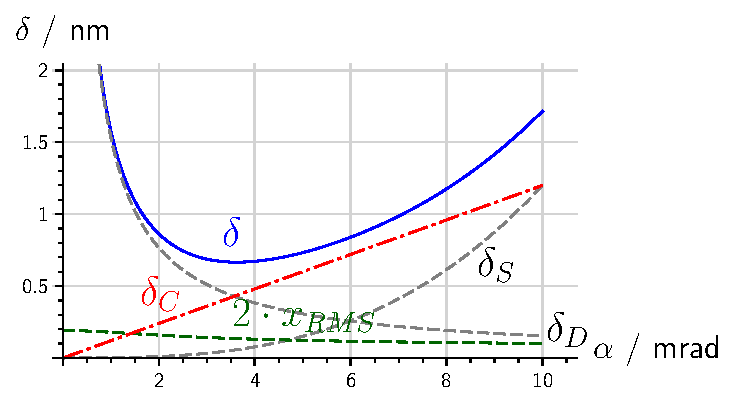
\includegraphics[width=.49\textwidth]{../Jupyter-Notebooks/AnhangC/Bilder/delta_TM_20eV_585eV+S}
		\label{fig:delta_TM_mit}
	}
	\caption{Auflösungsvermögen von ESI in Abhängigkeit vom Öffnungswinkel $\alpha$, berechnet nach \cite{thomas_introduction_2002} (Parameter: $C_S = \SI{1,2}{mm}$, $C_C = \SI{1,2}{mm}$, $\Delta E = \SI{718}{eV}$, $\delta E=\SI{20}{eV}$, $E=\SI{200}{keV}$ und somit $\lambda\approxeq \SI{2,51}{pm}$).}
\end{figure}

Die Relevanz des Farbfehlers steigt jedoch, wenn man Elementverteilungsbilder aufnimmt. Die Intensität konzentriert sich nicht mehr auf einen einzelnen Peak, sondern sie verteilt sich relativ gleichmäßig auf das mit der Spaltblende selektierte Energieverlustintervall. $\delta E$ nimmt entsprechend mit der Breite der Spaltblende (in \si{eV}) zu. Abbildung \ref{fig:delta_TG_20eV} zeigt die Radien der Fehlerscheiben für $\delta E=\SI{20}{eV}$. Für $\alpha=\SI{5,8}{mrad}$ vergrößert sich $\delta$ von \SI{0,353}{nm} auf \SI{0,782}{nm}, was einer Verschlechterung um mehr als den Faktor 2 entspricht.

Bisher bestimmen nur die Objektivlinse und die Objektivblende das Auflösungsvermögen. Hinzu kommt jedoch, dass die inelastische Anregung eines Atoms nicht lokalisiert erfolgt. Es gibt eine Abhängigkeit der Anregungswahrscheinlichkeit vom Abstand $b$ des Strahlelektrons zum angeregten Elektron. Um diese Abhängigkeit zu bestimmen, ist ein Zwischenschritt notwendig. Mit

\begin{align}
\Theta_E = \frac{\Delta E}{2 E} \label{eq:char_Winkel}
\end{align}

lässt sich der charakteristische Streuwinkel $\Theta_E$ zu einem Energieverlust $\Delta E$ bestimmen. Mit Hilfe von Energie- und Impulserhaltung erhält man unter Berücksichtigung von Gl. \ref{eq:char_Winkel}

\begin{align}
\Delta k^2(\Theta) = \frac{2\si{\electronmass}E}{\hbar^2}\left( \Theta_E^2 + \Theta^2 \right)\,.
\end{align}

Aus der Unschärferelation $\Delta b \approx \frac{1}{\Delta k}$ folgt nach einer kurzen Rechnung \cite[Appendix]{pennycook_high_1982}

\begin{align}
b_{RMS} = \frac{\hbar v \alpha}{\Delta E} \left[\left(\alpha^2+\Theta_E^2\right)\ln\left(\frac{\alpha^2}{\Theta_E^2}+1\right)\right]^{-\frac{1}{2}}\,. \label{eq:Delokalisation}
\end{align}

In \cite{thomas_introduction_2002} (bzw. \cite{krivanek_spatial_1995}) wird argumentiert, dass der Öffnungfehler keinen Einfluss auf die Wahl der Aufnahmeparameter hat. Damit lässt sich das \glqq vereinfachte theoretische Auflösungsvermögen\grqq\ bestimmen mit

\begin{align}
\delta_\mathrm{total} = \sqrt{\left(2\cdot b_\mathrm{RMS}\right)^2 + d_c^2 + d_b^2}\,. \label{eq:delta_TM}
\end{align}

Abbildung \ref{fig:delta_TM_ohne} zeigt das \glqq vereinfachte theoretische Auflösungsvermögen\grqq\ nach Gl. \ref{eq:delta_TM} in Abhängigkeit vom Öffnungswinkel $\alpha$. Zum Vergleich wird in Abbildung \ref{fig:delta_TM_mit} das theoretische Auflösungsvermögen unter Berücksichtigung des Öffnungsfehlers gezeigt. Für große Öffnungswinkel ist ein deutlicher Unterschied zu erkennen, jedoch würde eine optimale Wahl des Öffnungswinkels dazu führen, dass der Einfluss des Öffnungsfehlers vernachlässigbar ist.

\begin{figure}
	\centering
	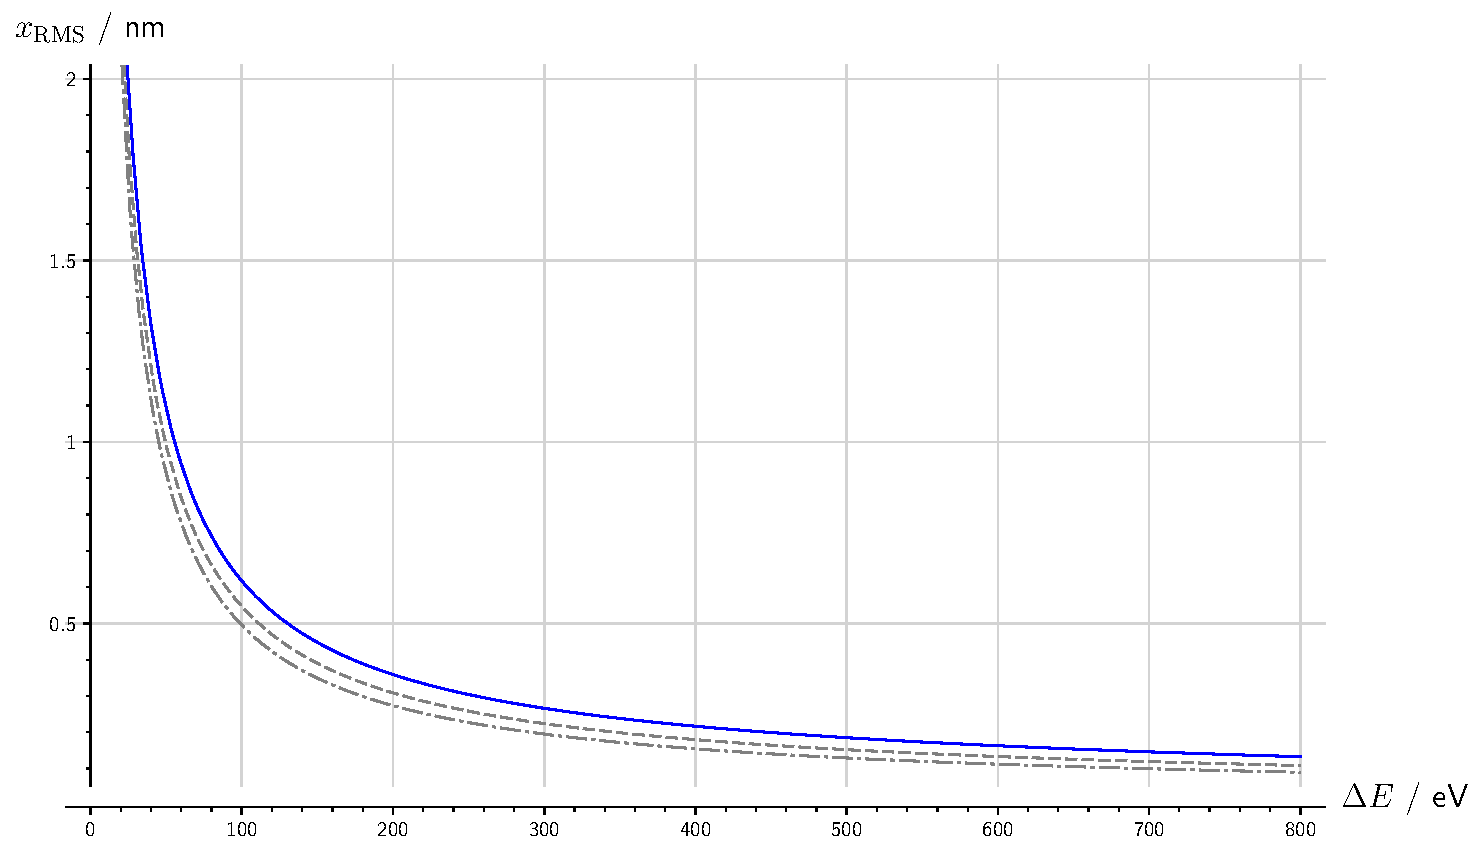
\includegraphics[width=1\linewidth]{../Jupyter-Notebooks/AnhangC/Bilder/delta_TM_loss}
	\caption{Abhängigkeit der Delokalisation vom Energieverlust. Es sind Kurven für 3 verschiedene Objektivblendendurchmesser zu sehen: $\SI{10}{\micro m} \mathrel{\hat=} \SI{2,9}{mrad}$ (blau), \SI{20}{\micro m} und \SI{40}{\micro m}}
	\label{fig:delta_TM_loss}
\end{figure}

Die Abhängigkeit der Delokalisation vom Öffnungsfehler ist sehr gering, da der charakteristische Streuwinkel $\Theta_E$ klein gegenüber dem Öffnungswinkel ist. Die Abhängigkeit der Delokalisation von Energieverlust $\Delta E$ ist deutlich größer. Abbildung \ref{fig:delta_TM_loss} zeigt $x_\mathrm{RMS}(E)$ in Abhängigkeit vom Energieverlust $\Delta E$.

Aus der Abbildung \ref{fig:delta_TM_loss} lässt sich entnehmen, dass für Energieverluste unterhalb von \SI{100}{eV} eine deutliche Verschlechterung der Ortsauflösung zu erwarten ist. Von V. Stolojan et al. gibt es jedoch einen Artikel, der zeigt, dass dies nicht für die Lokalisierung von Schichtgrenzen gilt \cite{stolojan_energy_2006}. Die in dieser Arbeit untersuchten Schichtsysteme aus Chrom und Eisen sollten somit auch bei Betrachtung der M-Kanten (\SI{42}{eV} bei Chrom und \SI{54}{eV} bei Eisen) mit hoher Ortsauflösung ($<\SI{1}{nm}$) analysiert werden können.

\section{Intensität als limitierender Faktor}

\begin{figure}
	\centering
	\subfloat[\SI{10}{\mu\meter}]{%
		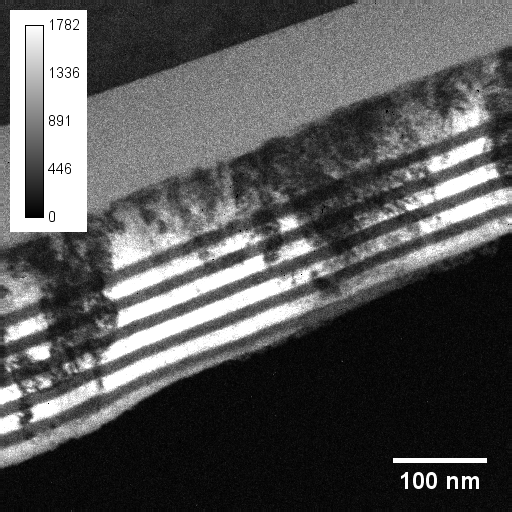
\includegraphics[width=.49\textwidth]{Bilder/ESI_Objektivblende_580eV_10mu}
		\label{fig:ESI_Objektivblende_580eV_10mu}
	}
	\subfloat[\SI{80}{\mu\meter}]{%
		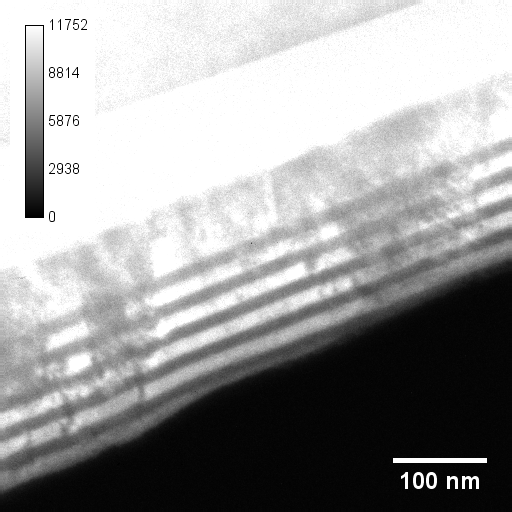
\includegraphics[width=.49\textwidth]{Bilder/ESI_Objektivblende_580eV_80mu}
		\label{fig:ESI_Objektivblende_580eV_80mu}
	}
	\caption[ESI Aufnahmen bei einem Energieverlust von \SI{580}{eV}]{ESI Aufnahmen bei einem Energieverlust von \SI{580}{eV} (Energieintervall: \SIrange{575}{595}{eV}). Es wurden die sieben verfügbaren Objektivblenden verwendet. Die beiden Abbildungen zeigen die kleinste Objektivblende (\SI{10}{\mu\meter}), sowie die größte Objektivblende (\SI{80}{\mu\meter}). Die Darstellung der Intensität wurde so gewählt, dass ein Bereich innerhalb der dritten durchgehenden Chrom-Schicht bei beiden Bildern gleich hell erscheint.}
	\label{fig:ESI_Objektivblende_580eV}
\end{figure}

\begin{figure}
	\centering
	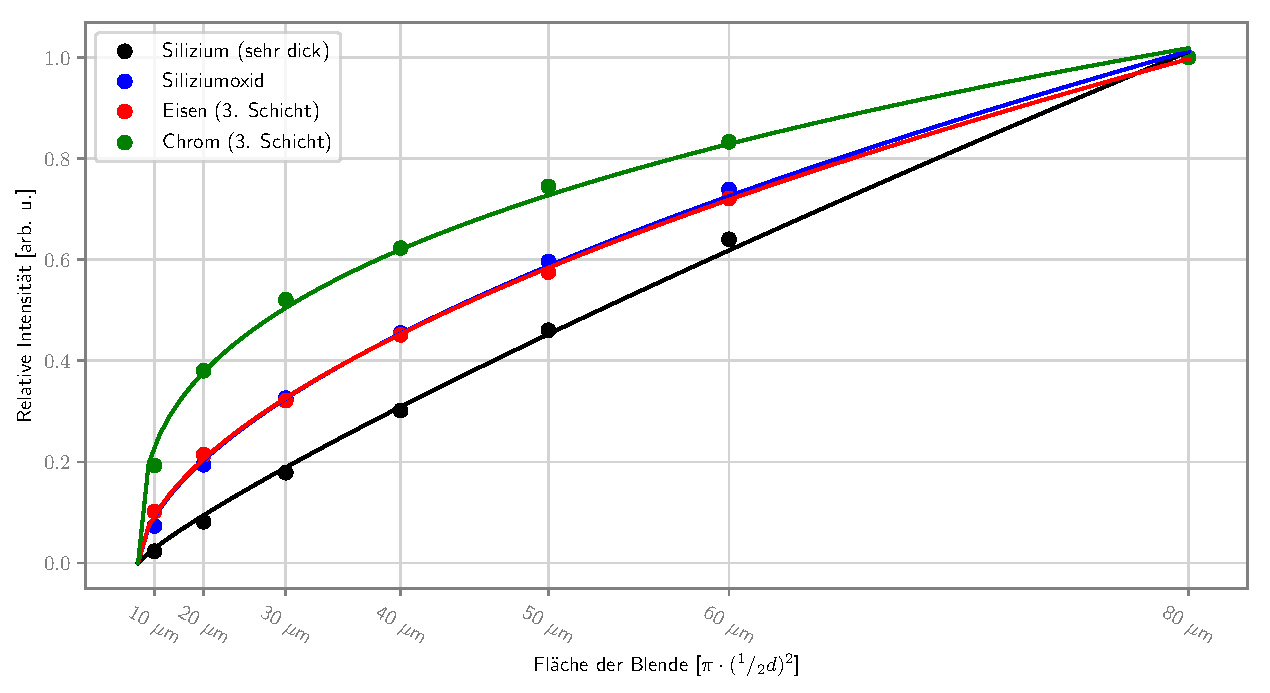
\includegraphics[width=1\linewidth]{../Jupyter-Notebooks/AnhangC/Bilder/ESI_Objektivblende}
	\caption{Abhängigkeit der mittleren Intensität von der Wahl der Objektivblende. Die einzelnen Kurven beziehen sich auf Bildbereiche, die jeweils ein einzelnes Element zeigen. Mit Hilfe von Abbildung \ref{fig:ESI_Objektivblende_580eV} können die Bildbereiche zugeordnet werden.}
	\label{fig:ESI_Objektivblende}
\end{figure}

\begin{table}
	\centering
	\caption{Intensität in Abhängigkeit vom Durchmesser der Objektivblende. Es sind die Messwerte gezeigt, die normiert in Abbildung \ref{fig:ESI_Objektivblende} genutzt werden. Neben dem Durchmesser der Blende ist der resultierende Öffnungswinkel aufgeführt (Brennweite: $f_\mathrm{O}=\SI{1,72}{mm}$).}
	\begin{tabular}{|r|r|r|r|}
		\hline 
		Blende & $\alpha_\mathrm{A}$ & Chrom & Eisen (BG) \\ 
		\hline 
		\SI{80}{\mu\meter} & \SI{23,3}{mrad} & 11108 & 6230 \\ 
		\hline 
		\SI{60}{\mu\meter} & \SI{17,4}{mrad} & 9251 & 4492 \\ 
		\hline 
		\SI{50}{\mu\meter} & \SI{14,5}{mrad} & 8275 & 3583 \\ 
		\hline 
		\SI{40}{\mu\meter} & \SI{11,6}{mrad} & 6917 & 2810 \\ 
		\hline 
		\SI{30}{\mu\meter} & \SI{8,7}{mrad} & 5784 & 1999 \\ 
		\hline 
		\SI{20}{\mu\meter} & \SI{5,8}{mrad} & 4224 & 1335 \\ 
		\hline 
		\SI{10}{\mu\meter} & \SI{2,9}{mrad} & 2145 & 634 \\ 
		\hline 
	\end{tabular} 
	\label{tab:ESI_Objektivblende}
\end{table}

Bisher wurde das Auflösungsvermögen nur in Bezug auf die Eigenschaften der Linsen betrachtet. Dabei stellte sich heraus, dass eine kleine Objektivblende (zum Beispiel \SIlist{10;20}{\mu\meter} beim Zeiss Libra 200FE) die beste mögliche Vergrößerung liefert. Gleichzeitig sinkt mit dem Durchmesser der Objektivblende auch das gemessene Signal. Dazu wurden mehrere ESI Aufnahmen gemacht, welche sich nur durch die verwendete Objektivblende unterscheiden. Das Ergebnis ist in Tabelle \ref{tab:ESI_Objektivblende} und Abbildung \ref{fig:ESI_Objektivblende} zu sehen. Im optimalen Fall sinkt die Intensität an der L$_{2,3}$-Kante nur auf \SI{20}{\percent} ab (dritte Chrom-Schicht), wenn man statt der \SI{80}{\mu\meter}- die \SI{10}{\mu\meter}-Blende verwendet. An den Werten für Eisen, Siliziumoxid und Silizium ist zu erkennen, dass das Untergrundsignal deutlich stärker abfällt. Bei der dritten Eisen-Schicht bleiben noch etwa \SI{10}{\percent} der maximalen Intensität. Für das Bestimmen des Element-Signals ist es von Vorteil, dass das Verhältnis von Signal zu Untergrund ansteigt. Leider hat das Absinken der Gesamtintensität auch Nachteile. Um eine weiterhin geringe relative Unsicherheit (Poisson-Statistik: $\sigma_\mathrm{rel}=\frac{1}{\sqrt{N}}$) bei Aufnahme mit kleinerer Objektivblende zu erhalten, muss die Belichtungszeit erhöht werde.

Auf diese Weise entsteht ein komplexer Parameter-Raum, den es zu optimieren gilt, um optimale Ergebnisse zu erzielen. Details zu dieser Optimierung sind in den Artikeln von A.\ Berger und H.\ Kohl zu finden \cite{berger_optimum_1993,berger_detection_1994,kohl_resolution_1995}. In dieser Arbeit soll jedoch nicht genauer darauf eingegangen werden.

\clearpage

\bibliographystyle{myamsalpha}
\bibliography{Literatur}

\end{document}